\item Two interacting particles form a closed system whose centre of inertia is at rest. Fig. 1.36 illustrates the positions of both particles at a certain moment and the trajectory of the particle of mass $m_1$. Draw the trajectory of the particle of mass $m_2$ if $m_2 = m_1/2$.
    \begin{center}
        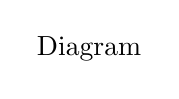
\begin{tikzpicture}
            \node at (0, 0) {Diagram};
        \end{tikzpicture}
    \end{center}\begin{solution}
    \begin{center}
        \begin{tikzpicture}
            \pic at (0, 0) {frame=3cm};
        \end{tikzpicture}
    \end{center}
    
    \begin{align*}
        \intertext{As the closed system consisting of two particles $m_1$ and $m_2$ is initially at rest, the centre of mass of the system will remain at rest. Further as $m_2 = m_1/2$, the centre of mass of the system divides the line joining $m_1$ and $m_2$ at all the moments of time in the ratio 1:2. In addition to it, the total linear momentum of the system at all the times is zero.}
        \vec{p}_1 &= -\vec{p}_2 
        \intertext{and therefore the velocities of $m_1$ and $m_2$ are also directed in opposite sense. Bearing in mind all these things, the sought trajectory is as shown in the figure.}
    \end{align*}
\end{solution}